% Related Work (Priyanshu)
% Uses \relevance and projectbox from main.tex. Every paper fact was checked against the paper itself,
% its DOI / proceedings page or its official data record. Our numbers come from reports/results_table.md.
% Figure: figures/rw_context_ladder.png.

\section{Related Work}
\label{sec:related}

We review the literature in four steps: the physics-based model that learned models aim to replace,
machine learning in wildfire science, learned spread models on NDWS and related datasets, and the methods
our pipeline is built on. Table~\ref{tab:relwork} compares the spread studies, and
Section~\ref{sec:rw_position} places our work among them.

\subsection{Physics-based fire spread}

\textbf{Rothermel~\cite{rothermel1972}} developed the surface fire spread model that still underlies U.S.\
fire behaviour tools. Andrews~\cite{andrews2018} describes it as quasi-empirical. It combines a heat-balance
formulation with wind-tunnel experiments in artificial fuel beds and grassfire observations. The model
computes the steady-state rate of spread of a fire front through a uniform fuel bed. Its inputs are fuel
load, depth, surface-area-to-volume ratio, heat content, mineral content, moisture and moisture of
extinction, together with midflame wind speed and slope. It was first used in the 1972 U.S.\ National
Fire Danger Rating System (NFDRS) and is built into BehavePlus and FARSITE~\cite{andrews2018}.
\relevance{} the energy release component (\texttt{erc}) in our data is an NFDRS output. Our features
use the same drivers (wind, slope, dryness), but leave the form of the relationship to the learner.

\subsection{Machine learning in wildfire science}

\textbf{Jain et al.~\cite{jain2020}} review machine learning in wildfire science and management. They find
300 publications up to the end of 2019. Fire occurrence, susceptibility and risk is the largest domain
(127 papers), and fire behaviour prediction, which includes spread, has 43. Random forests, MaxEnt,
neural networks, decision trees, SVMs and genetic algorithms are the most common methods.
\relevance{} spread prediction is a small part of the field.

\textbf{Sayad et al.~\cite{sayad2019}} predict wildfire \emph{occurrence} from three MODIS products (NDVI,
land surface temperature, thermal anomalies) over central Canada. Their table has 804 rows (386 fire, 418
no fire), and an ANN and an SVM reach 98.32\% accuracy. \relevance{} with balanced classes, accuracy is
informative. On our test split, 98.75\% of pixels do not burn, so accuracy is not.

\subsection{Learned spread models on other data}

\textbf{Hodges and Lattimer~\cite{hodges2019}} train a deep convolutional inverse graphics network to
reproduce simulated burn maps (Rothermel's equations and FARSITE) every 6\,h up to 24\,h. They report
precision, sensitivity, F-measure and Chan-Vese similarity of 0.97, 0.92, 0.93 and 0.93 against the
simulator, at a computational cost three orders of magnitude lower. \relevance{} these scores measure
agreement with a simulator, not with observed fires.

\textbf{Radke et al.~\cite{radke2019}} (FireCast) predict 24\,h spread from GeoMAC perimeters of Rocky
Mountain fires since 2013, Landsat-8 imagery, elevation and weather, using a CNN on a window around each
pixel. On the 2016 Beaver Creek fire they report 87.7\% accuracy and 91.1\% recall, but 3.6\% precision
and a 6.4\% F-score. \relevance{} when fire is rare, accuracy and recall can hide very low precision.

\textbf{Gerard et al.~\cite{gerard2023}} build WildfireSpreadTS, a multi-day dataset of 13\,607 VIIRS
images (375\,m) of 607 U.S.\ fires from 2018 to 2021, scored by average precision over 12 year-based folds.
Persistence reaches 0.193, logistic regression up to 0.288, a ResNet-18 U-Net 0.341, and a temporal
attention U-Net (UTAE) with five input days 0.372. \relevance{} a different sensor and split, but the same
ordering: spatial and temporal models beat pixel models.

\subsection{Learned spread models on NDWS}

\textbf{Huot et al.~\cite{huot2022}} introduce Next Day Wildfire Spread (NDWS): 18\,545 fire events over
the contiguous U.S.\ (2012-2020), each a $64\times64$\,km patch at 1\,km with 12 day-$t$ inputs and the
day-$(t{+}1)$ MODIS fire mask. Whole weeks are assigned to train, eval and test in an 8:1:1 ratio. On PR
AUC, persistence scores 0.115, logistic regression 0.198, and a random forest of depth 15 scores 0.225;
both pixel models see each pixel and its eight neighbours. A convolutional autoencoder that sees the
whole patch reaches 0.284. \relevance{} we use their data, split and metric.

\textbf{Fitzgerald et al.~\cite{fitzgerald2023}} add attention blocks to a U-Net and train it with focal
loss on random $32\times32$ crops, discarding crops with uncertain labels. The best model reaches F1
0.370; no PR AUC is reported. They also note that most next-day fire lies in the patch centre and that
models learn to predict fire there. \relevance{} cropped, filtered test sets give numbers that cannot be
compared with full-patch results.

\textbf{Xiao et al.~\cite{xiao2024}} propose an attention U$^2$-Net and report F1 0.405. They re-split
all 18\,545 samples at random 8:1:1 instead of using the official week-based split, and fill uncertain
labels with 0. \relevance{} a random re-split can place samples of the same fire in training and test.

\textbf{Andrianarivony and Akhloufi~\cite{andrianarivony2025}} (LinU-Mamba) use the official split and
report F1 $42.22 \pm 0.29$ over 10 runs, with uncertain labels clamped to 0 and no PR AUC. Retraining
earlier models on the full split, they find much lower F1 than those papers reported on subsets (20.06
instead of 70.97 for a multi-kernel CNN~\cite{marjani2023}). \relevance{} evaluation protocol changes the
numbers as much as the model does.

\textbf{Zhou et al.~\cite{zhou2025}} compare an autoencoder, ResNet, U-Net and Swin-UNet on $32\times32$
crops; the split is not stated. Swin-UNet reaches PR AUC 0.280 and U-Net 0.274, and an XGBoost baseline,
whose setup is not described, reaches 0.06. \relevance{} the only other tree model on NDWS we found; our
per-pixel XGBoost reaches 0.257 with engineered spatial features.

\textbf{Two recent preprints} report PR AUC on full patches with uncertain labels excluded.
\textbf{Esparza et al.~\cite{esparza2026}} use the official split, choose the threshold on training and
eval data only, and give bootstrap intervals. Their re-run of the convolutional autoencoder reaches 0.327
and a U-Net 0.346, and their best ensemble 0.379. \textbf{Han et al.~\cite{han2026}} (FireSenseNet) report
PR AUC 0.3435, but choose their F1 threshold on the test set. They also show that predicting the union of
both days' fire and setting uncertain labels to 0 inflate F1 by 44-50\%, as in~\cite{luo2026}.
\relevance{} these are the closest comparisons to our protocol, but neither is peer-reviewed.

\begin{table*}[t]
\centering
\caption{Spread studies at a glance. Only rows with the same data, split and metric are comparable; the
protocol column gives the differences. Preprints are marked $^\dagger$.}
\label{tab:relwork}
\small
\setlength{\tabcolsep}{4pt}
\renewcommand{\arraystretch}{1.12}
\newcolumntype{L}[1]{>{\raggedright\arraybackslash}p{#1}}
\begin{tabular}{L{3.4cm}L{3.6cm}L{5.0cm}L{1.9cm}L{2.3cm}}
\toprule
\rowcolor{tblhead}
\textbf{Paper} & \textbf{Method} & \textbf{Data / protocol} & \textbf{Metric} & \textbf{Result} \\
\midrule
Hodges \& Lattimer 2019~\cite{hodges2019} & CNN (DCIGN) & simulated burn maps & F vs.\ simulator & 0.93 \\
Radke et al.\ 2019~\cite{radke2019} & CNN + weather & GeoMAC/Landsat-8, Rocky Mts.\ & Precision / recall & 3.6\% / 91.1\% \\
Gerard et al.\ 2023~\cite{gerard2023} & U-Net / UTAE & WildfireSpreadTS, VIIRS 375\,m & AP & 0.341 / 0.372 \\
\midrule
Huot et al.\ 2022~\cite{huot2022} & Persistence / LR / RF & NDWS official split; LR, RF use 3$\times$3 window & PR AUC & 0.115 / 0.198 / 0.225 \\
Huot et al.\ 2022~\cite{huot2022} & Conv.\ autoencoder & NDWS official split & PR AUC & 0.284 \\
Zhou et al.\ 2025~\cite{zhou2025} & U-Net / Swin-UNet / XGBoost & NDWS, $32\times32$ crops, split not stated & PR AUC & 0.274 / 0.280 / 0.06 \\
Esparza et al.\ 2026$^\dagger$~\cite{esparza2026} & Conv.\ AE / U-Net & NDWS official split, full patches & PR AUC & 0.327 / 0.346 \\
Han et al.\ 2026$^\dagger$~\cite{han2026} & Dual-branch CNN & NDWS 8:1:1, F1 threshold on test & PR AUC & 0.3435 \\
Fitzgerald et al.\ 2023~\cite{fitzgerald2023} & Attention U-Net & NDWS, $32\times32$ crops, uncertain crops dropped & F1 & 0.370 \\
Xiao et al.\ 2024~\cite{xiao2024} & Attention U$^2$-Net & NDWS random re-split, uncertain $\to$ 0 & F1 & 0.405 \\
Andrianarivony \& Akhloufi 2025~\cite{andrianarivony2025} & LinU-Mamba & NDWS official split, uncertain $\to$ 0 & F1 & 0.422 \\
\rowcolor{tblours}
\textbf{Ours} & \textbf{XGBoost, 35 features} & \textbf{NDWS official split, full patches} & \textbf{PR AUC} & \textbf{0.257} \\
\bottomrule
\end{tabular}
\end{table*}

\subsection{Methods we build on}

\textbf{Gradient-boosted trees.} Friedman~\cite{friedman2001} frames boosting as gradient descent in
function space, with regression trees as base learners. Chen and Guestrin~\cite{chen2016} add a
regularised objective and second-order split finding in XGBoost, our main model. Ke et
al.~\cite{ke2017} speed up histogram-based boosting with gradient-based sampling and feature bundling in
LightGBM, our second model, which trains up to more than 20 times faster at similar accuracy. Breiman's
random forests~\cite{breiman2001} average decorrelated trees; they are the strongest pixel model of Huot et
al. Section~\ref{sec:theory_gb} explains how these ideas set our hyperparameters.

\textbf{Segmentation networks.} Ronneberger et al.~\cite{ronneberger2015} propose U-Net, an
encoder-decoder with skip connections for segmentation with few labelled images; it won the ISBI 2015
cell-tracking challenge on two datasets. It is the base of most NDWS models above and a candidate for our
Phase~2.

\textbf{Learning and evaluating under imbalance.} Focal loss~\cite{lin2017} down-weights easy examples,
the alternative to class weighting discussed in Section~\ref{sec:theory_imb}. Davis and
Goadrich~\cite{davis2006} prove that one curve dominates in ROC space if and only if it dominates in PR
space and that PR curves must not be interpolated linearly, and Saito and Rehmsmeier~\cite{saito2015}
show that ROC plots can mislead on imbalanced data. Both support PR AUC as our metric
(Section~\ref{sec:theory_pr}).

\textbf{Interpretation.} SHAP~\cite{lundberg2017} attributes a prediction to features with Shapley
values, and TreeSHAP~\cite{lundberg2020} computes them exactly for tree ensembles. Our Results section uses
them to check that the model's dependence on fire distance, dryness and wind is physically sensible.

\subsection{Where our work sits}
\label{sec:rw_position}

\begin{projectbox}
Three points stand out from Table~\ref{tab:relwork} and Fig.~\ref{fig:rw_ladder}.

\textbf{Protocols differ.} Crops, the handling of uncertain labels, splits and test-set thresholds change
the reported numbers. Only Huot et al.\ and Esparza et al.\ clearly use the official split with full
patches and PR AUC, the protocol we follow.

\textbf{Spatial features help trees.} The NDWS work we found is almost entirely deep spatial models.
Trees appear only as Huot et al.'s neighbour-window baselines (0.225) and as an XGBoost baseline at 0.06. Our
per-pixel XGBoost with engineered spatial features reaches 0.257, above both, and the ablation traces this
to the fire-neighbourhood features.

\textbf{Spatial models are still ahead.} Huot et al.'s CNN (0.284) and recent U-Nets (0.346 in a
preprint) score higher. This gap is what motivates Phase~2: a spatial model that sees the whole patch and
the shape of the fire front. As in the papers above, we have not checked whether one fire can appear in
more than one split.
\end{projectbox}

\begin{figure}[t]
\centering
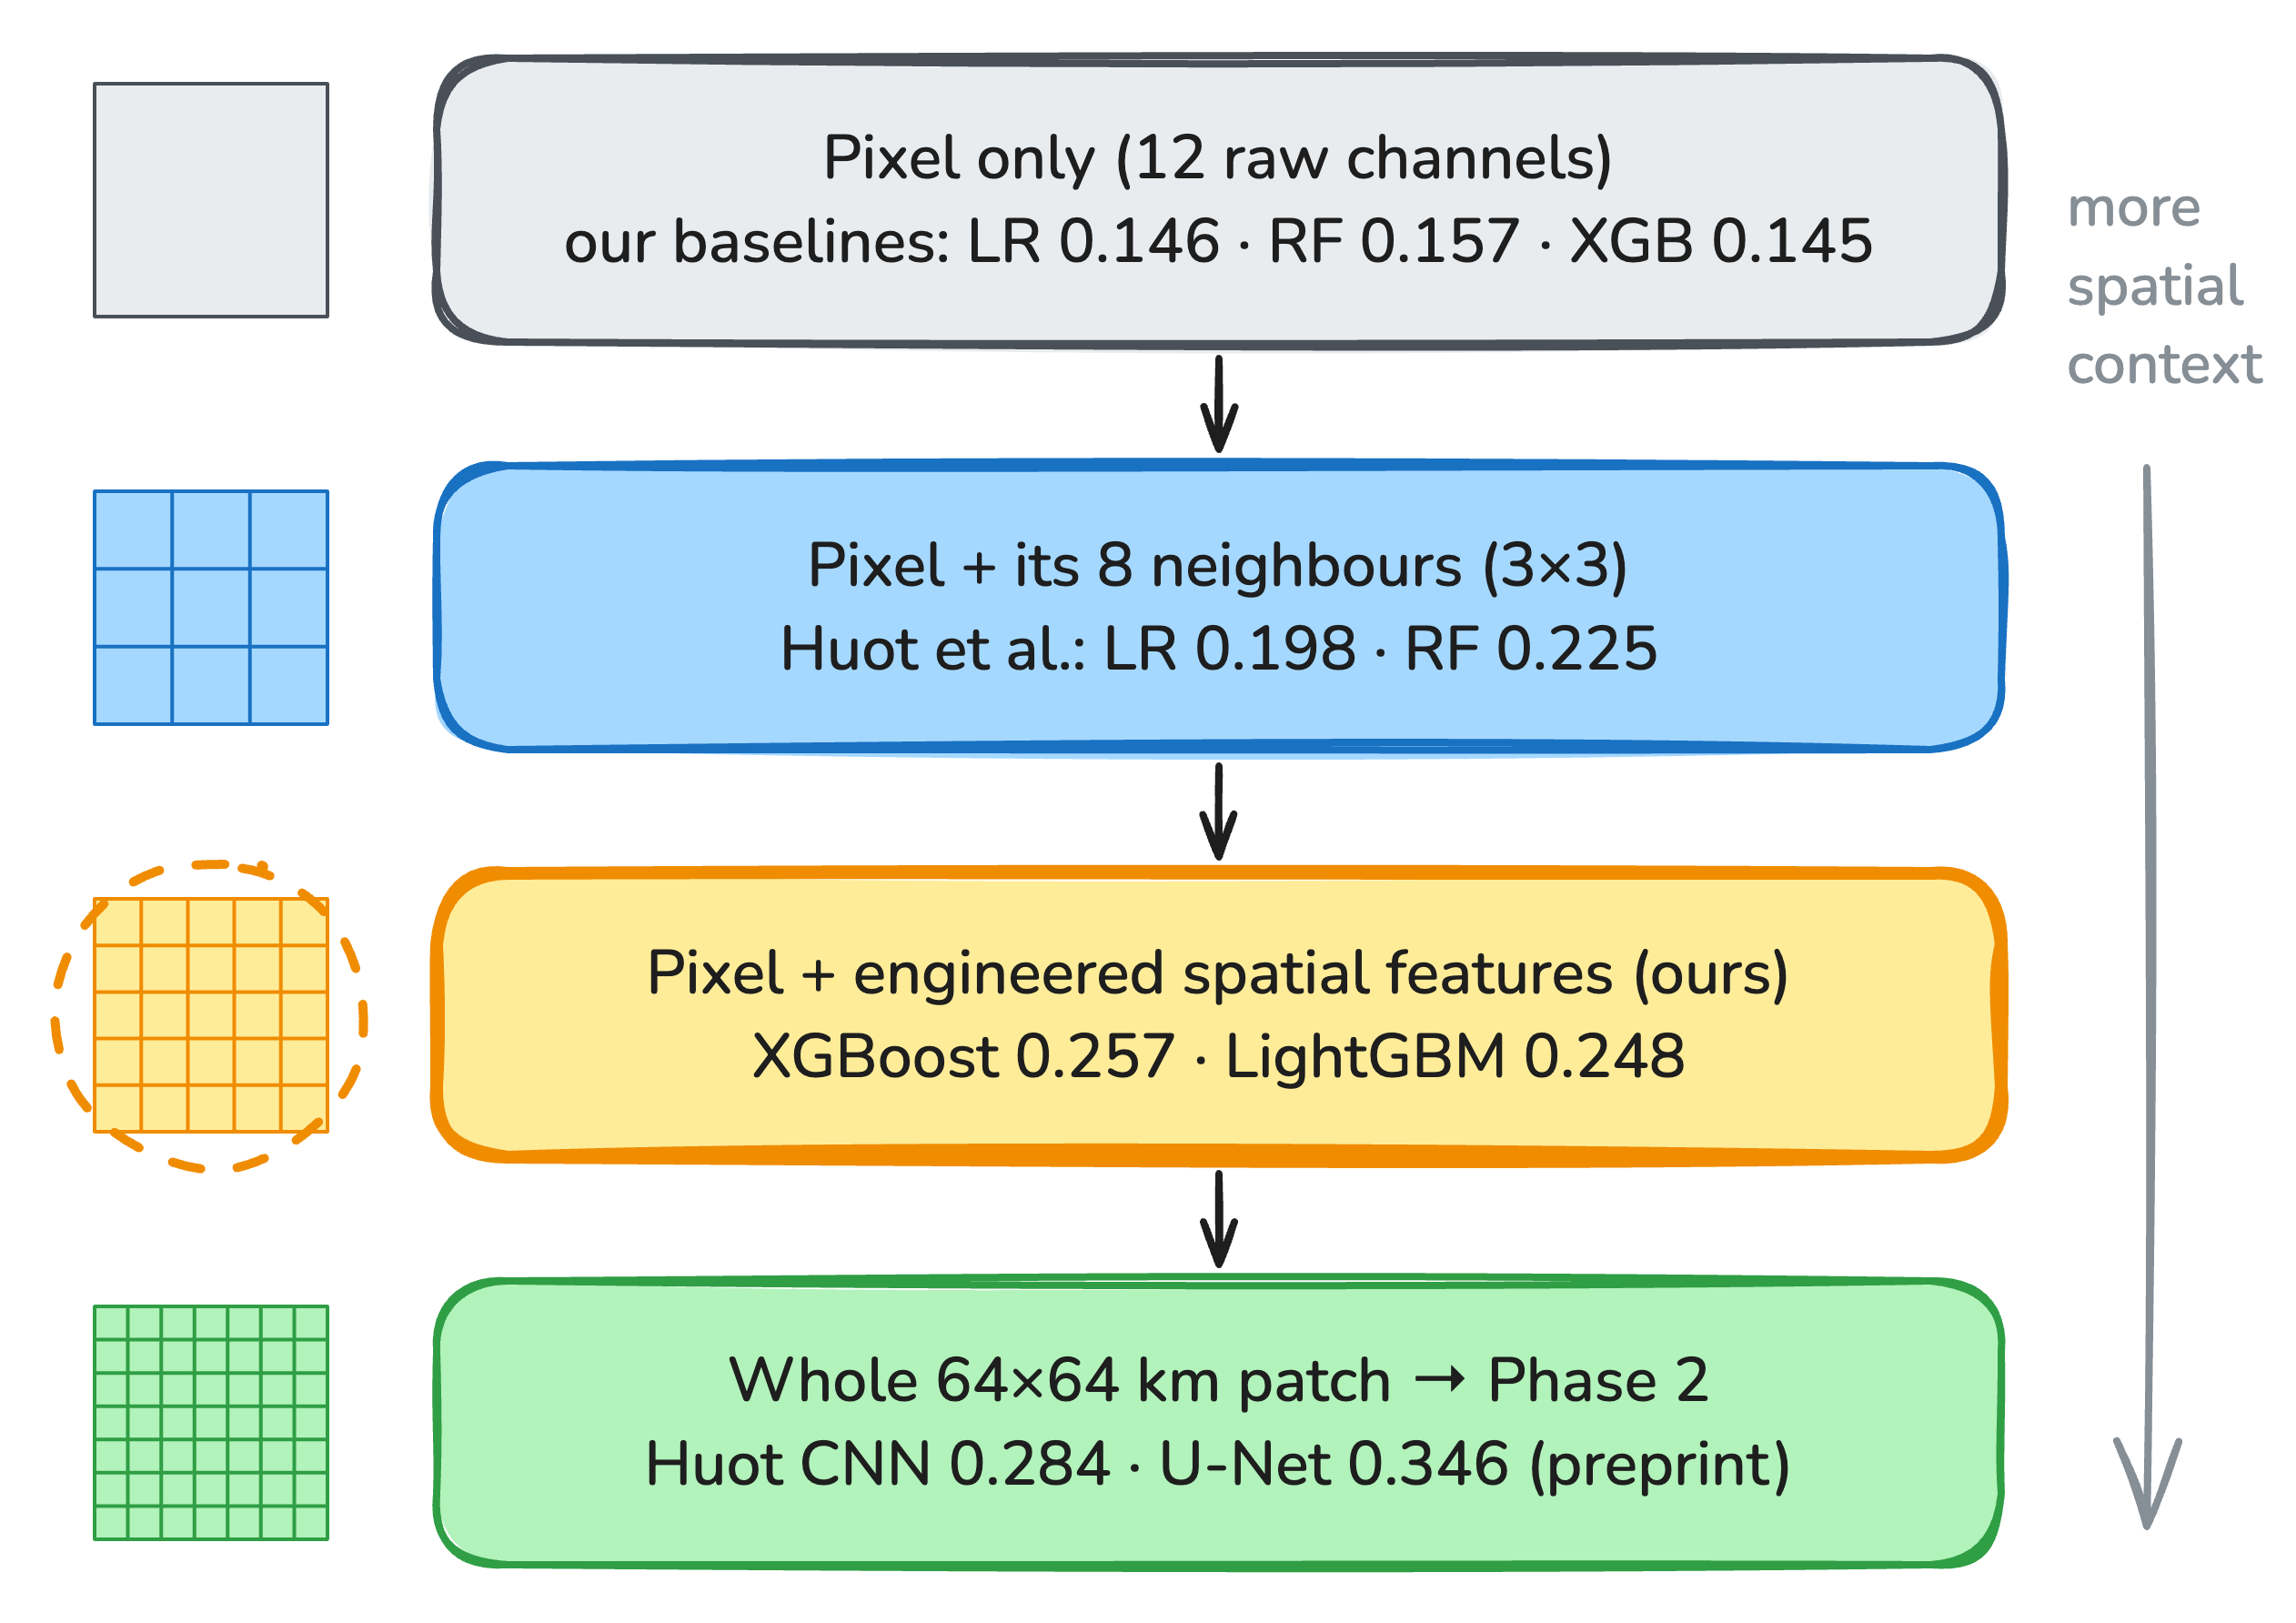
\includegraphics[width=\columnwidth]{figures/rw_context_ladder.png}
\caption{NDWS models ordered by the spatial context they see, with test PR AUC. Raw-channel baselines are
ours; the others are from~\cite{huot2022,esparza2026}.}
\label{fig:rw_ladder}
\end{figure}
